\chapter{研究の準備}\label{cha:Preparation}
本章では、\toolName を試作する際に必要な前提知識について説明する。
なお、本論文では、Webページを構成する要素を、
画面要素\cite{Element}と呼ぶ。画面要素として、本研究で扱うHTMLタグの例を、表\ref{tb: HTML_tag}に示す。
\begin{table}[tp]
      \caption{Webページの画面要素として扱うHTMLタグの例}
      \label{tb: HTML_tag}
      \centering
      \begin{tabular}{c|l}
            \hline
            HTMLタグ                     & \multicolumn{1}{c}{説明}  \\
            \hline \hline
            $<$div$>$                    & \begin{tabular}{l}セッションやレイアウトのブロックを形成するコンテナを表すタグ。\end{tabular} \\ \hline
            $<$h1$>~<$h6$>$             & \begin{tabular}{l}見出しタグ。$<$h1$>$が最も重要な見出しを表すタグ。\\$<$h6$>$へと重要度が下がっていく。\end{tabular} \\ \hline
            $<$p$>$                      & \begin{tabular}{l}テキストの段落を定義するタグ。\end{tabular} \\ \hline
            $<$a$>$                      & \begin{tabular}{l}ハイパーリンクを表すタグ。他のページや同ページ内の別のセクションへの\\リンクを提供する。\end{tabular} \\ \hline
            $<$img$>$                    & \begin{tabular}{l}画像の埋め込みを表すタグ。\end{tabular} \\ \hline
            $<$ul$>$, $<$ol$>$, $<$li$>$ & \begin{tabular}{l}箇条書きリストを定義するタグ。\end{tabular} \\ \hline
            $<$form$>$                   & \begin{tabular}{l}ユーザからの入力を受け取るためのフォームを表すタグ。\end{tabular} \\ \hline
            $<$input$>$                  & \begin{tabular}{l}ユーザからのデータ入力を受け取るための入力フィールドを表すタグ。\end{tabular} \\ \hline
            $<$button$>$                 & \begin{tabular}{l}ユーザがクリックできるボタンを表すタグ。\end{tabular} \\ \hline
      \end{tabular}
\end{table}

\section{視覚的回帰テスト}\label{sec:vrt}
視覚的回帰テスト(Visual Regression Testing)\cite{VisualRegressionTesting}は、
開発者の意図しないレイアウトの差分、すなわち、レイアウトの不具合が発生していないことを確認するテスト手法である。
特に、Webページを対象とした視覚的回帰テストは、変更前後のWebページを並べて、レイアウトの差分を強調表示することで、
レイアウトの差分を発見しやすくする。
% なお、本研究では、比較対象とするWebページの画像を「比較画像」、テスト対象とするWebページの画像を「テスト画像」と定義する。
\par
Webページを対象とした視覚的回帰テストの基本的な手順は、以下の通りである。
\begin{enumerate}
      \setlength{\itemsep}{0pt}
            \setlength{\parsep}{0pt}
      \item 変更前画像の取得:\\
            テスト対象とするWebページの画面をスクリーンショットする。この画像を、変更前画像とする。
      \item 変更の適用:\\
            テスト対象とするWebページに、画面要素の追加や削除、編集を適用する。
      \item 変更後画像の取得:\\
            変更したテスト対象とするWebページの画面をスクリーンショットする。この画像を、変更後画像とする。
      \item 画像比較に基づくレイアウトの差分検出:\\
            変更前画像と変更後画像を比較し、レイアウトの差分を検出する。
            % 一部の視覚的回帰テストツール\cite{}は、2つの画像をピクセル単位で比較し、差分を強調表示する。
      \item 結果の評価:\\
            差分検出の結果を確認し、検出したレイアウトの差分が意図した差分であるかどうかを判定する。
            レイアウトの不具合が発生していた場合、HTMLコードの修正を行い、再度テストを行う。
\end{enumerate}

\section{レイアウトの不具合箇所}\label{sec:layout effect}
% レイアウトの不具合\cite{LayoutFailureDetection}箇所とは、Webページの画面要素が適切にレイアウトされていない画面要素のことである。
レイアウトの不具合箇所の定義とそれに関する定義を、以下に示す。
\begin{itemize}
      \item 差分箇所:\\
            変更前後のWebページの画像を比較して、変更前のWebページから削除された範囲と、
            変更後のWebページに追加された範囲。
      \item 変更箇所:\\
            変更前後のWebページのHTMLコードを比較して、HTMLコードにおけるbody要素内の変更とstyle要素内の変更のどちらか、
            または両方が適用された画面要素の範囲。
            本研究では、変更箇所を意図的なレイアウトの差分の範囲とみなす。
      \item レイアウトの不具合箇所:\\
            差分箇所から、意図的なレイアウトの差分の範囲であるHTMLコードの変更箇所を除いた、
            レイアウトの不具合の範囲。
\end{itemize}
% \begin{itemize}
%       \item 差分箇所:\\
%             Webページの変更前画像とWebページの変更後画像を比較して、
%             変更前のWebページから削除された範囲と変更後のWebページに追加された範囲を可視化する。
%       \item 変更箇所:\\
%             変更前後のWebページのHTMLコードを比較して、
%             HTMLコードにおけるbody要素内の変更とstyle要素内の変更のどちらか、
%             または両方の変更が適用された画面要素の範囲を可視化する。
%             本研究では、変更箇所を意図的に変更した範囲と見なす。
%       \item レイアウトの不具合箇所:\\
%             差分箇所から、意図的に変更した範囲であるHTMLコードの変更箇所を除いた、
%             意図しない差分の範囲を可視化する。
% \end{itemize}
\par
レイアウトの不具合箇所には、開発者が意図せず隠れてしまう画面要素や重なってしまう画面要素が存在する。
例えば、レイアウトの不具合箇所によって、以下のような状態が起こりうる。
\begin{itemize}
      \setlength{\itemsep}{0pt}
            \setlength{\parsep}{0pt}
      \item 画面要素のはみ出し:\\
            Webページの画面要素が、ブラウザの表示画面外や、$<$div$>$タグ(表\ref{tb: HTML_tag}を参照)で
            構成されるコンテナ外に一部または完全にはみ出している。                 
      \item 画面要素の重なり:\\
            Webページの画面要素が、他の固定された画面要素の上に重なっている。
\end{itemize}
画面要素のはみ出しの例を図\ref{fig:hamidasi}に、画面要素の重なりの例を図\ref{fig:overlap}に、それぞれ示す。
図\ref{fig:hamidasi}は、変更前画像上の白いコンテナ内で3番目のテキストが、変更後画像上で白いコンテナ外に一部はみ出している。
図\ref{fig:overlap}は、変更前画像上の白いコンテナ内で下のテキストが、変更後画像上でフッターと重なっている。
\begin{figure}[tp]
      \begin{center}
            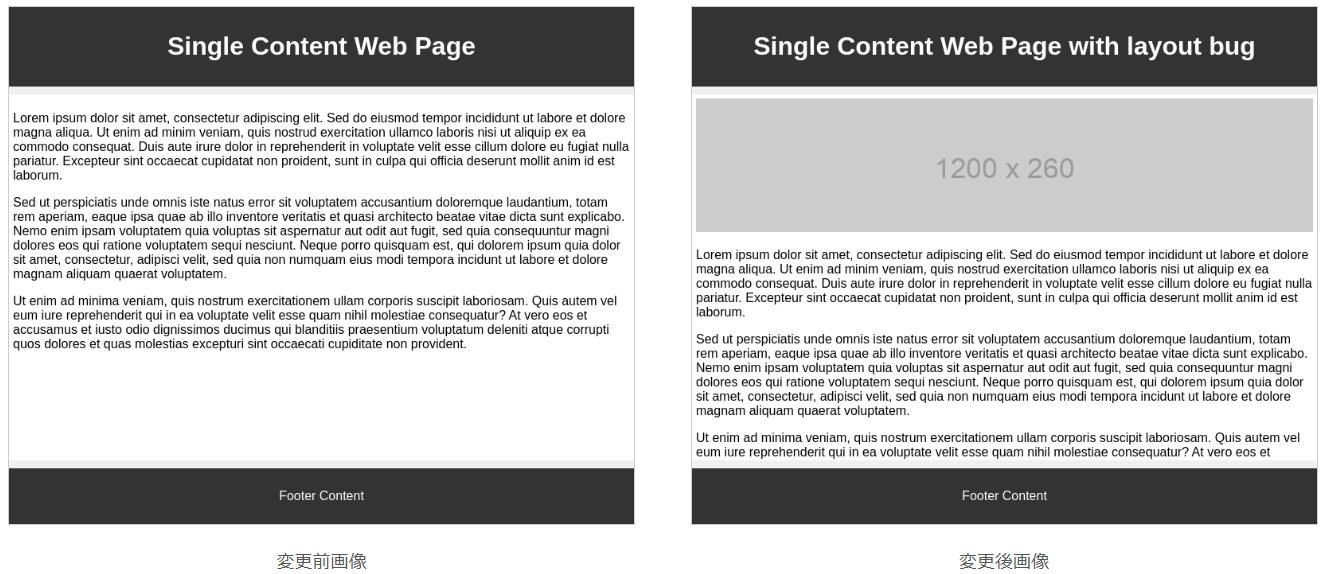
\includegraphics[width=1.0\columnwidth]{image/2/hamidasi.png}
            \caption{画面要素のはみ出しの例}
            \label{fig:hamidasi}
      \end{center}
\end{figure}
\begin{figure}[tp]
      \begin{center}
            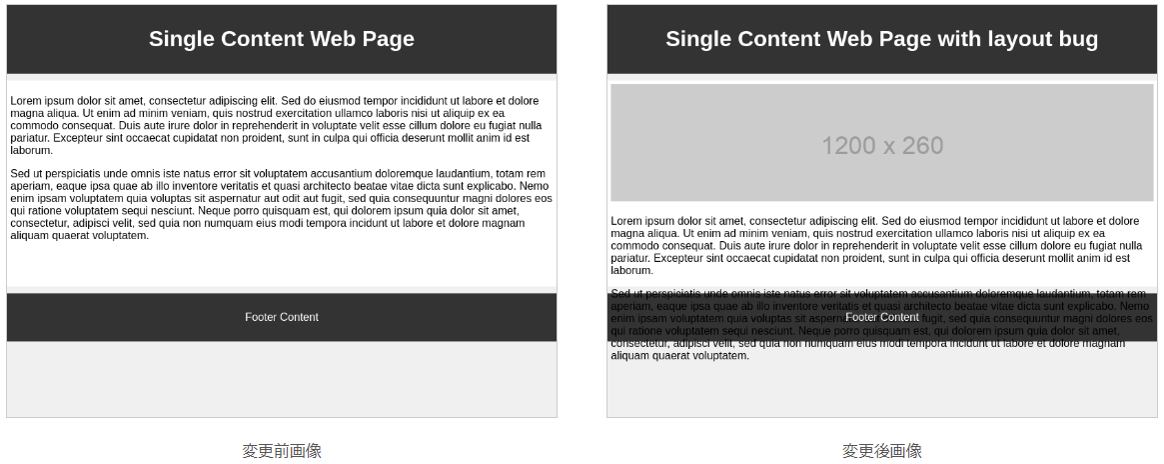
\includegraphics[width=1.0\columnwidth]{image/2/overlap.png}
            \caption{画面要素の重なりの例}
            \label{fig:overlap}
      \end{center}
\end{figure}
\par
図\ref{fig:hamidasi}に示すように、画面要素のはみ出しは視認できないこともあるため、WebページのHTMLコードを見て確認し、修正する必要がある。
また、レイアウトの不具合箇所は、元々HTMLコード内に存在した不適切な実装が、新しく追加や編集を行った他の画面要素の影響で表面化する場合がある。
そのため、Webページを変更した開発者にも発見しづらいという特徴がある。
% レイアウトの不具合箇所の定義とそれに関する定義を、以下に示す。
% \begin{itemize}
%       \item 差分箇所:\\
%             Webページの変更前画像と変更後画像を比較して、
%             変更前のWebページから削除された画面要素と変更後のWebページに追加された画面要素。
%       \item 変更箇所:\\
%             変更前後のWebページのHTMLコードを比較して、
%             HTMLコードにおけるbody要素内の変更とstyle要素内の変更のどちらか、
%             または両方の変更が適用された画面要素。
%       \item レイアウトの副作用箇所:\\
%             Webページの変更前画像と変更後画像で、変更箇所によって、
%             HTMLコードを変更していない画面要素にレイアウトの変更があった画面要素。
%       \item レイアウトの不具合箇所:\\
%             レイアウトの副作用箇所のうち、画面要素のはみ出し、見切れ、重なりがあった画面要素。
% \end{itemize}

% 本研究では、画面要素の隠れ、見切れ、重なりの3つのレイアウトの不具合箇所を、以下の方法で検出する。
% \begin{enumerate}
%       \item 差分箇所から変更箇所を取り除くことで、レイアウトの副作用箇所を抽出する
%       \item レイアウトの副作用箇所から、変更前後で画面要素の見た目が変わっていない画面要素を取り除くことで、
%             レイアウトの不具合箇所を抽出する
% \end{enumerate}

% \par
% 上記3つのレイアウトの不具合例として、画面要素のはみ出しを埋め込んだWebページの変更前画像と変更後画像を図\ref{fig: hide_element}に、
% 画面要素の見切れを埋め込んだWebページの変更前画像と変更後画像を図\ref{fig: crip_element}に、
% 画面要素の重なりを埋め込んだWebページの変更前画像と変更後画像を図\ref{fig: overlap_element}に、
% それぞれ示す。
% \begin{figure}[tp]
%       \begin{center}
%             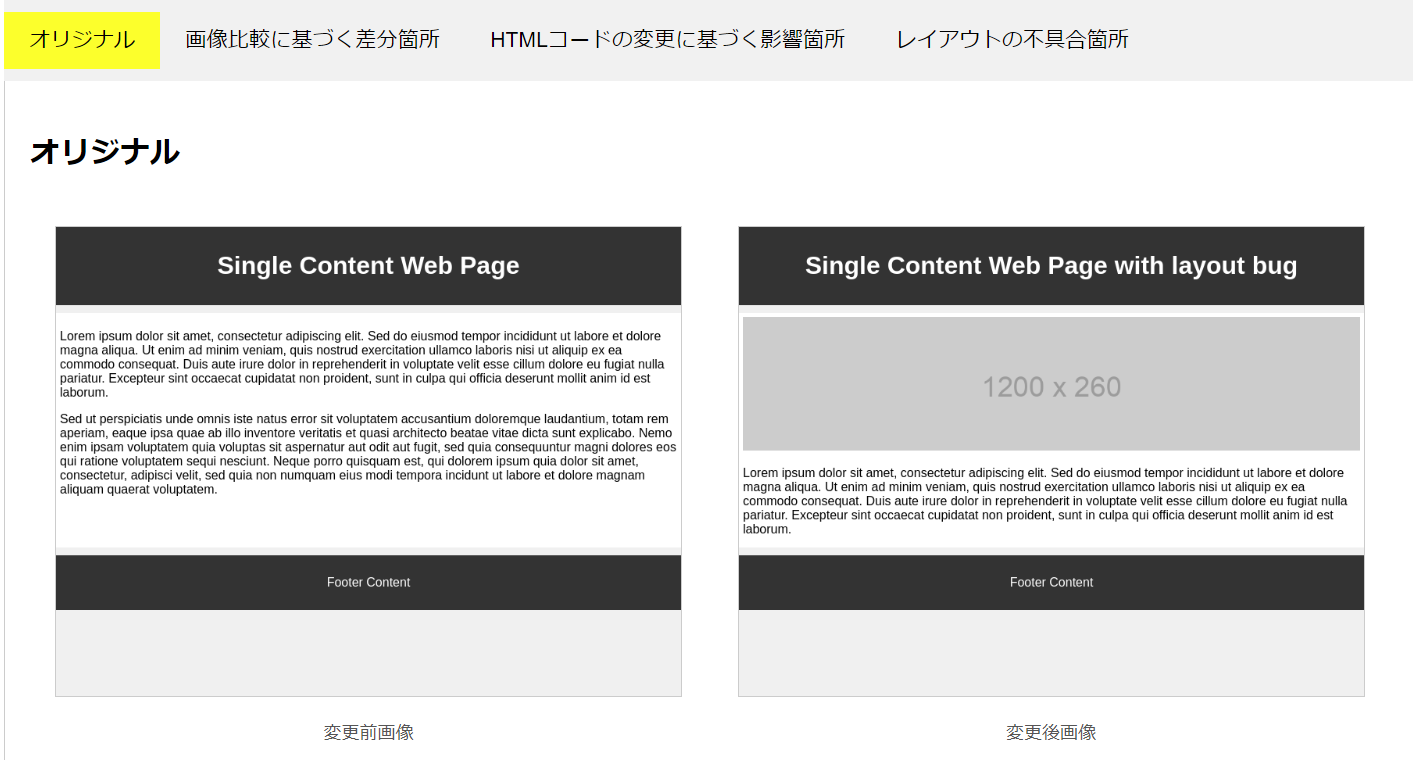
\includegraphics[width=1.0\columnwidth]{image/5/ex1_original.png}
%             \caption{画面要素のはみ出しを埋め込んだWebページの変更前画像と変更後画像}
%             \label{fig: hide_element}
%       \end{center}
% \end{figure}
% \par
% \begin{figure}[tp]
%       \begin{center}
%             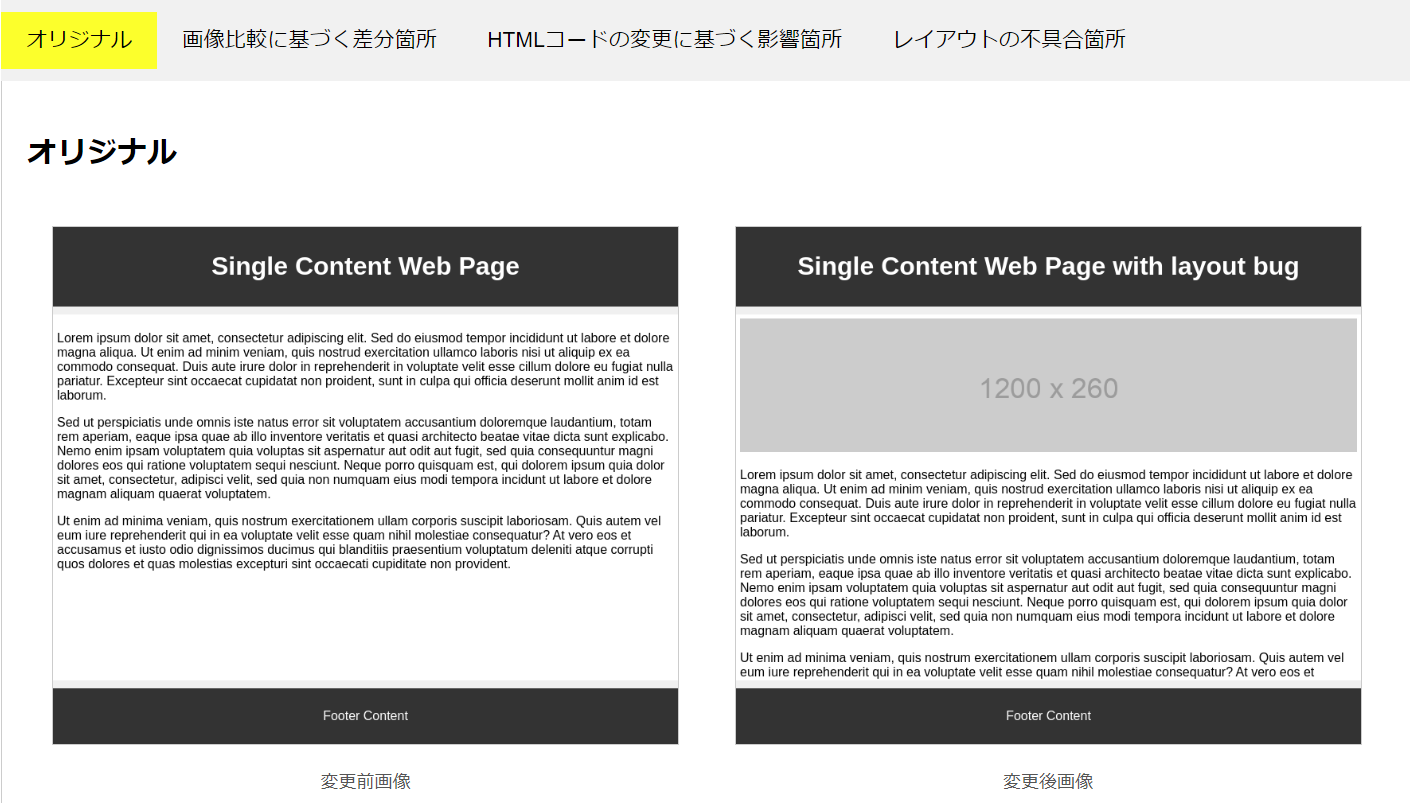
\includegraphics[width=1.0\columnwidth]{image/5/ex4_original.png}
%             \caption{画面要素の見切れを埋め込んだWebページの変更前画像と変更後画像}
%             \label{fig: crip_element}
%       \end{center}
% \end{figure}
% \begin{figure}[tp]
%       \begin{center}
%             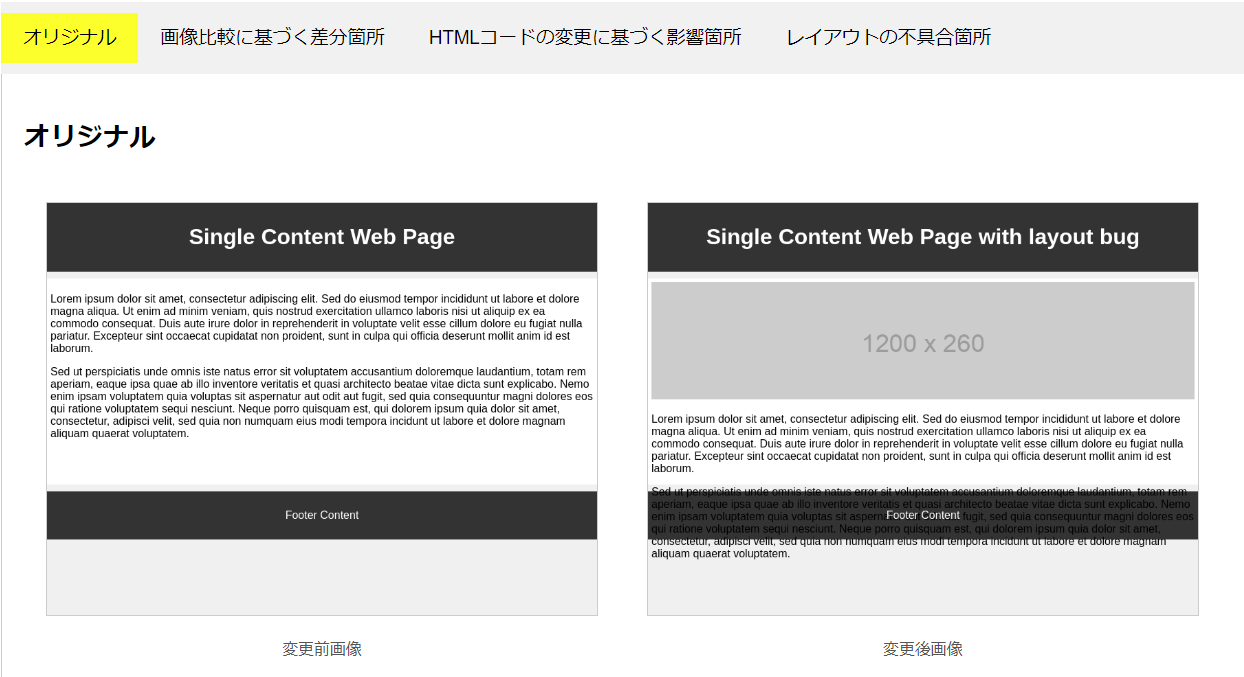
\includegraphics[width=1.0\columnwidth]{image/5/ex3_original.png}
%             \caption{画面要素の重なりを埋め込んだWebページの変更前画像と変更後画像}
%             \label{fig: overlap_element}
%       \end{center}
% \end{figure}

% また、以下の画面要素に対して、レイアウトの不具合を検出する。
% \begin{itemize}
%     \setlength{\itemsep}{0pt}
%           \setlength{\parsep}{0pt}
%     \item テキスト
%     \item 画像
%     \item ボタン
%     \item ヘッダー
%     \item フッター
% \end{itemize}
\section{OpenCV}\label{sec:opencv}
OpenCV (Open Source Computer Vision Library)\cite{OpenCV}は、画像や動画に関する処理機能をまとめた、コンピュータビジョン向けのオープンソースのライブラリである。
\par
本研究では、OpenCVに用意されている、imread関数、cvtColor関数、threshold関数、adaptiveThreshold関数、
subtract関数、dilate関数、findContours関数、boundingRect関数、rectangle関数、absdiff関数の10個の関数を用いる。
各関数について、以下で説明する。

\paragraph{imread関数}
imread関数は、画像ファイルの読み込みを行う関数である。
第一引数に、画像ファイルのパスを指定する。
% 読み込まれた画像ファイルは、OpenCVに用意されている関数を用いて画像処理を適用できる画像データとなる。
% 第二引数に、画像ファイルの読み込み方法を指定する。
% 読み込まれた画像データは、OpenCVで広く使われるデータ形式となる。
% これにより、OpenCVに用意されている関数を用いて、画像処理を適用できる。
\par
本研究では、グレースケール化や二値化処理などの画像処理を適用するために、
この関数を使用してWebページの画像や\toolName が生成する画像を読み込む。
\paragraph{cvtColor関数}
cvtColor関数は、画像の色空間を変換する関数である。
第一引数には、色空間の変換を適用する画像を指定し、第二引数には、どの色空間へ変換するかを示すコード\cite{ColorCode}を指定する。
\par
本研究では、画像処理の高速化と精度向上のために、
BGR(青、緑、赤)からGRAY(グレースケール)への色空間の変換を行う。
また、画像処理の適用で削除された画面要素や追加された画面要素を検出した際、色で識別可能にするために、GRAY(グレースケール)からBGR(青、緑、赤)への色空間の変換を行う。
\paragraph{threshold関数}
threshold関数は、画像を二値化する関数である。
第一引数には、グレースケール画像を指定し、第二引数には、二値化する際の閾値を指定する。
第三引数には、ピクセル値の最大値を指定し、第四引数には、二値化の方法を指定する。
\par
本研究では、二値化の方法として、閾値以下のピクセル値をピクセルの明度の最大値($255$)に変換し、
それ以外のピクセル値を$0$に変換する二値化方法であるcv2.THRESH\_BINARY\_INV\cite{Threshold}を設定する。
\paragraph{adaptiveThreshold関数}
adaptiveThreshold関数は、画像を複数の小さな区画に切り分けた各々の部分に異なる閾値を用いて画像の二値化を行う関数である。
第一引数には、二値化を適用するグレースケール画像を指定し、第二引数には、二値化後のピクセルにおける明度の最大値を指定する。
第三引数には、二値化の閾値を計算する方法を指定し、第四引数には、二値化の方法を指定する。
第五引数には、近傍領域のサイズを指定し、
第六引数には計算された二値化の閾値から引かれる定数を指定する。
\par
本研究におけるadaptiveThreshold関数は、画像の一部が明るく、他の部分が暗い場合においても、均一な二値化画像を生成するために用いる。
\par
また、本研究において、adaptiveThreshold関数の第三引数から第六引数に関しては、以下の値を設定する。
\begin{itemize}
      \setlength{\itemsep}{0pt}
            \setlength{\parsep}{0pt}
      \item 二値化の閾値を計算する方法:\\
            近傍領域内のピクセル平均値(近傍領域内のピクセル合計値 $\div$ 近傍領域内のピクセル数)に基づいて閾値を計算するcv2.ADAPTIVE\_THRESH\_MEAN\_C\cite{AdaptiveThreshold}に設定する。
      \item 二値化の方法:\\
            threshold関数でも用いたcv2.THRESH\_BINARY\_INV\cite{Threshold}に設定する。
      \item 近傍領域のサイズ:\\
            $11$(ピクセル)に設定する。
      \item 計算された二値化の閾値から引かれる定数:\\
            $2$に設定する。
\end{itemize}
% \paragraph{bitwise\_not関数}
% bitwise\_not関数は、画像の各ピクセル値のビットを反転する関数である。
% ビット反転の例として、黒ピクセル($0$のピクセル値)は白ピクセルに(ピクセル値が$255$に)、白ピクセル($255$のピクセル値)は黒ピクセルに(ピクセル値が$0$に)反転する。
% 第一引数にビット反転を行う画像を指定する。
\paragraph{subtract関数}
subtract関数は、2つの画像間の対応するピクセル値を比較し、差分画像を返す関数である。
第一引数には、比較の基準となる画像を指定する。
第二引数には、第一引数の画像と比較する画像を指定する。第二引数で指定した画像の各ピクセル値が、第一引数で指定する画像の対応するピクセル値から引かれる。
% (例: 二値化前の画像AとBが元々Webページの画像であり、Webページ内のテキストやボタンなどの画面要素が二値化後の画像で白ピクセル、それ以外の背景などが黒ピクセル領域となっている画像)
例として、二値化画像AとBはそれぞれ白ピクセルに特徴がある画像とし、
subtract関数の第一引数に二値化画像Aを、
第二引数に二値化画像Bを、それぞれ指定した場合のsubtract関数のピクセル値の比較処理を、以下に示す。
\par
\begin{itemize}
      \setlength{\itemsep}{0pt}
            \setlength{\parsep}{0pt}
      \item 共通の白ピクセル:\\
            二値化画像AとBの両方で白ピクセルの場合、subtract関数は$255$(Aの白ピクセル値)から$255$(Bの白ピクセル値)を引く。
            差は$0$(黒ピクセル値)になり、共通の白ピクセルは黒ピクセルとなる。
      \item Aのみに存在する白ピクセル:\\
            二値化画像Aは白ピクセルで、二値化画像Bは黒ピクセルの場合、subtract関数は$255$(Aの白ピクセル値)から$0$(Bの黒ピクセル値)を引く。
            差は$255$(白ピクセル値)になり、Aのみに存在する白ピクセルはそのまま残る。
      \item Bのみに存在する白ピクセル:\\
            二値化画像Aは黒ピクセルで、二値化画像Bは白ピクセルの場合、subtract関数は$0$(Aの黒ピクセル値)から$255$(Bの白ピクセル値)を引く。
            差は$-255$になるが、subtract関数は負の値を$0$(黒ピクセル値)として処理するため、Bのみに存在する白ピクセルは黒ピクセルとなる。
      \item 共通の黒ピクセル:\\
            二値化画像AとBの両方で黒ピクセルの場合、subtract関数は$0$(Aの黒ピクセル値)から$0$(Bの黒ピクセル値)を引く。
            差は$0$(黒ピクセル値)になり、共通の黒ピクセルはそのまま黒ピクセルとなる。
\end{itemize}
上記の処理の結果、二値化画像Aのみに存在する白ピクセルを抽出した差分画像が生成できる。
\par
本研究では、二値化処理を行ったWebページの変更前画像と変更後画像のそれぞれに対して、交互に1回ずつsubtract関数の第一引数と第二引数に指定し実行することで、
変更前画像から削除された画面要素を抽出した差分画像と、変更後画像に追加された画面要素を抽出した差分画像の2つの差分画像を生成する。
\paragraph{dilate関数}
dilate関数は、二値化画像内の白ピクセルに対して膨張処理を行う関数であり、ノイズ除去や、オブジェクトの形状とサイズの強調に役立つ。
膨張処理は、カーネルと呼ばれる特定のサイズと形状の小さなフィルタを使用する。このフィルタを画像上でスライドし、各ピクセルに対して
フィルタ内の最大値を割り当てていくことで、白ピクセルを拡大する。
第一引数に、膨張処理を行う画像を指定する。
第二引数に、カーネルのサイズと形状を指定する。
第三引数に、膨張処理の適用回数を指定する。
\par
本研究において、dilate関数の第二引数と第三引数に関しては、以下の値を設定する。
\begin{itemize}
      \setlength{\itemsep}{0pt}
            \setlength{\parsep}{0pt}
      \item カーネルのサイズと形状:\\
            5 $\times$ 5ピクセルの正方形に設定する。
      \item 膨張処理の適用回数:\\
            $6$に設定する。
\end{itemize}
\par
本研究におけるdilate関数は、subtract関数で生成した差分画像内の、
削除された画面要素または追加された画面要素の形状とサイズを強調する。
それにより、変更箇所と同等の粒度で、
後述するrectangle関数が、削除された画面要素と追加された画面要素を枠で囲むことを目的としている。
% この目的の結果、差分箇所と変更箇所の比較の際に、レイアウトの副作用箇所(\ref{cha:Function}章で後述)の検出精度を高めることができる。
% 差分箇所(\ref{cha:Function}章で後述)を枠で囲む粒度を、変更箇所(\ref{cha:Function}章で後述)を枠で囲む粒度に近づけることができるため、
% レイアウトの不具合箇所の検出に役立つ。
% 本研究では、差分箇所を枠で囲む粒度を、変更箇所を枠で囲む粒度と合わせるために用いる。
\paragraph{findContours関数}
findContours関数は、画像から輪郭を検出し、検出した各輪郭の輪郭データを格納する輪郭リストを返す。
第一引数に輪郭抽出の対象画像(通常は二値化画像)を指定する。
第二引数に輪郭構造の取得方法を指定する。
第三引数に、輪郭の形成方法を指定する。
\par
本研究において、findContours関数の第二引数と第三引数に関しては、以下の値を設定する。
\begin{itemize}
      \setlength{\itemsep}{0pt}
            \setlength{\parsep}{0pt}
      \item 輪郭構造の取得方法:\\
            画像内の一番外側の白の輪郭のみを取得するRETR\_EXTERNAL\cite{RetrExternal}に設定する。
      \item 輪郭の形成方法:\\
            端点のみで輪郭を形成するCHAIN\_APPROX\_SIMPLE\cite{ChainApproxSimple}に設定する。
\end{itemize}
\par
% また、本研究におけるfindContours関数は、後述するboundingRect関数で
% Webページの変更前画像から削除された箇所の輪郭座標を、
% Webページの変更後画像に追加された箇所の輪郭座標を取得するために、輪郭データを取得する。
\paragraph{boundingRect関数}
boundingRect関数は、輪郭データをもとに、その輪郭を完全に囲む最小の矩形(バウンディングボックス)を計算する関数である。
第一引数は、findContours関数で取得した輪郭リストの各要素である輪郭データを指定する。
% なお、輪郭データは、単一の輪郭を表す配列であり、この配列に輪郭を形成する点の集合を含む。
\par
本研究におけるboundingRect関数は、矩形の左上隅画素のx座標とy座標、さらに矩形の幅と高さを取得するために用いる。
これにより、輪郭を取り囲む矩形の位置とサイズを取得できる。
なお、画像の座標系は、画像の左上隅画素を原点 (0,0) とし、右方向をX軸の正の向き、下方向をY軸の正の向きと定義する。
\paragraph{rectangle関数}
rectangle関数は、画像に矩形を描画する関数である。
第一引数に描画先の画像、第二引数に矩形の左上の点の座標、第三引数に矩形の右下の点の座標、
第四引数に矩形の色、第五引数に矩形の線の太さを指定する。
\par
本研究におけるrectangle関数は、画像上の指定した位置に、指定した大きさと色の矩形を描画し、特定の領域を視覚的に強調するために用いる。
\paragraph{absdiff関数}
absdiff関数は、2つの配列または画像間における絶対値の差を計算する関数である。
第一引数に、1つ目の入力配列または画像を指定する。
第二引数に、2つ目の入力配列または画像を指定する。なお、第二引数は、第一引数の入力配列または画像と同じサイズ、かつ、同じデータ型にする必要がある。
\par
本研究におけるabsdiff関数は、入力された2つの配列または画像間における各ピクセル値の絶対値の差を計算し、
その結果を出力配列または画像として返すために用いる。

\section{Pillow}\label{sec:pillow}
Pillow\cite{Pillow}は、プログラミング言語Python\cite{Python}の画像処理ライブラリの1つで、画像の読み込み、画像処理操作、保存などの機能を提供する。
\par
本研究では、Pillowに用意されている、Image.open関数\cite{ImageModule}とリサンプリングフィルタであるImage.LANCZOS\cite{LANCZOS}を用いる。
なお、本研究におけるImage.open関数とImage.LANCZOSは、画像比較部の高解像度画像生成処理(\ref{subsec:Generate_high_images}節で後述)の際に、
変更前画像と変更後画像から、変更前高解像度画像と変更後高解像度画像を生成するために用いる。
\paragraph{Image.open関数}
Image.open関数は、指定したパスの画像ファイルを開き、PillowライブラリにおけるImageクラスのインスタンスを生成して返す。
このImageクラスのインスタンスに対して、画像のサイズ変更、回転、色調整など、様々な画像処理操作が可能である。
\paragraph{Image.LANCZOS}
Image.LANCZOSは、画像のサイズ変更時に使用されるリサンプリングフィルタの1つである。
LANCZOSフィルタは、画像を拡大する際に細部やエッジを維持できるため、高解像度画像の生成処理に適している。
\par

\section{NumPy}\label{sec:numpy}
NumPy\cite{NumPy}は、Pythonにおいて数値計算を効率的に行うためのパッケージである。
効率的な数値計算を行うための型付き多次元配列のサポートをPythonに加えるとともに、それらを操作するための大規模な高水準の数学関数ライブラリを提供する。
\par
本研究では、NumPyに用意されている、numpy.zeros関数\cite{np.zeros}を用いる。
\paragraph{numpy.zeros関数}
numpy.zeros関数は、指定した形状とデータ型を持つ、すべての要素が$0$の新しい配列を生成する関数である。
第一引数に、生成する配列の形状を指定する。
第二引数に、配列のデータ型を指定する。
なお、配列の形状とは、生成する配列の次元数と各次元数における要素数のことである。
\par
本研究におけるnumpy.zeros関数は、$0$で初期化した画像(黒画像)を生成するために用いる。

\section{Selenium WebDriver}\label{sec:Selenium_WebDriver}
Selenium WebDriver\cite{SeleniumWebDriver}は、Seleniumプロジェクト\cite{Selenium}の一部であり、Webブラウザを直接制御するためのAPIを提供する。
Selenium WebDriverのAPIを用いてテストスクリプトを実行することで、指定したWebページにアクセスし、要素のクリックやページ遷移などのユーザ操作を自動で行う。

\section{requests}\label{sec:requests}
requests\cite{Requests}は、PythonでHTTPリクエストを扱うためのライブラリである。
Webサイトへのアクセス、データ送受信、セッション管理、クッキー操作、SSL認証を可能にする。
開発者がHTTPを簡単に扱えるように、HTTP/1.1\cite{HTTP}規格に基づき設計されている。

\section{BeautifulSoup}\label{sec:beautifulsoup}
BeautifulSoup\cite{BeautifulSoup}は、HTMLやXMLファイルからデータを取り出すためのPythonライブラリである。
このライブラリを利用することで、タグの検索や属性の取得、テキストの抽出などを容易に行うことができる。
\par
本研究では、BeautifulSoupに用意されている、find\_all関数とget\_text関数を用いる。
\paragraph{BeautifulSoupの初期化}
BeautifulSoupに用意されている関数を用いるには、まず、BeautifulSoupオブジェクトを初期化する必要がある。
BeautifulSoupオブジェクトとは、HTMLデータを解析し、操作可能な形式に変換したデータ構造である。
このオブジェクトの初期化には、解析するHTMLデータと使用するパーサーを指定する。
\par
本研究では、使用するパーサーに、HTMLデータを解析するパーサーである“html.parser”\cite{BeautifulSoup}を用いる。
\paragraph{find\_all関数}
find\_all関数は、引数で指定したタグに一致するすべての要素を検索し、それらをリストとして返す。
リストには、HTMLやXMLファイルにおける検索された要素の行番号を格納する。
\paragraph{get\_text関数}
get\_text関数は、引数で指定したタグのテキスト内容を返す。

\section{difflib}\label{sec:difflib}
difflib\cite{difflib}は、Pythonで文字列を要素として格納するリスト間の差分を検出し、処理するための標準モジュールである。
本節では、文字列を要素として格納したリストを、文字列リストと呼ぶ。
% このモジュールは、異なるテキストデータ間の差分を識別し、それらの違いを詳細に比較する機能を提供する。
\par
本研究では、difflibに用意されているDifferクラスのメソッドを用いる。
\paragraph{Differクラス}
Differクラスは、2つの文字列リスト間の差分を行単位で計算し、詳細な差分情報を生成するためのクラスである。
このクラスは、文字列リストの各行を個別に比較し、追加、削除、変更された行を特定する。
\paragraph{compareメソッド}
compareメソッドは、Differクラスのインスタンスを使用して、2つの文字列リスト間の差分を計算する。
このメソッドは、2つの文字列リストを引数として受け取り、差分結果を行単位で返す。
差分結果には、追加された行が“+”記号で、削除された行が“-”記号で、変更のない行がスペースで行の先頭にマークされる。
また、“?”記号を用いて、変更があった行についての詳細な差分を示す。
\par
本研究では、差分コード生成処理(\ref{subsec:diff_file_generate}に後述)で生成する差分コードに関しては、
行の先頭が“?”記号から始まる行を除外する。これは、“?”記号で始まる行については、解析の対象としないためである。
% \begin{itemize}
%       \setlength{\itemsep}{0pt}
%             \setlength{\parsep}{0pt}
%       \item "- ":\\
%             行はシーケンス1のみに存在する。
%       \item "+ ":\\
%             行はシーケンス2のみに存在する。
%       \item "? ":\\
%             行は入力シーケンスのどちらにも存在しない(どの文字がどのように変更したかという差分の詳細)。
% \end{itemize}
% 差分コードの例を、ソースコード\ref{lst:diff_html_?}に示す。
% \begin{lstlisting}[language=HTML, caption=差分コードの例, label=lst:diff_html_?]
%   <header>
% -     <h1>Single Content Web Page</h1>
% +         <h1>Single Content Web Page with layout bug</h1>
% ?                                    ++++++++++++++++

%   </header>
% \end{lstlisting}

\section{Flask}\label{sec:Flask}
Flask\cite{Flask}は、プログラミング言語PythonでWebサーバやWebアプリを構築する際に用いられるWebフレームワークである。
このフレームワークは、Werkzeug\cite{Werkzeug}とJinja2\cite{Jinja}に基づいている。
Werkzeugは、WebサーバとWebアプリケーション間のリクエストやレスポンスを処理するWSGI(Web Server Gateway Interface)ツールキットである。
なお、WSGI\cite{WSGI}とは、WebサーバとWebアプリケーション間の接続規格である。
Jinja2は、Pythonで使用されるテンプレートエンジン\cite{TemplateEngine}で、Webページの動的なレンダリングを可能にする。
\par
本研究では、Flaskを用いてローカルサーバを構築し、以下を実現する。
\begin{itemize}
      \setlength{\itemsep}{0pt}
            \setlength{\parsep}{0pt}
      \item \toolName が生成した画像(\ref{subsec:MixVRT_IO}節で後述)を閲覧できるWebページを開発者に提供する。
      \item HTML比較部(\ref{sec:Affected_area_extraction}節で後述)で生成した枠付きHTMLコードをレンダリングし、
            Flaskを用いて立てたローカルサーバのURLへのアクセスを通じて、レンダリングを行った枠付きWebページを表示する。
\end{itemize}
なお、枠付きWebページを表示する目的は、Selenium WebDriverを用いて、
枠付きHTMLコードによるWebページの画像を取得するためである。

\section{\toolName の環境構築}\label{sec:MixVRT_env_gen}
\toolName の環境構築には、Dockerコンテナ\cite{DockerContainer}を使用する。
具体的には、ローカルサーバ用、Python処理用、およびSeleniumのGoogle Chrome用の、3つのDockerコンテナを使用する。
Docker Compose\cite{DockerCompose}を用いて、開発者はこれらのコンテナを同時に起動する。
\par
ローカルサーバ用コンテナは、Flaskを用いたローカルサーバを提供する。
Python処理用コンテナは、Pythonを用いた画像処理やHTMLコード解析処理を行う。
SeleniumのGoogle Chrome用コンテナは、Webブラウザの自動操作を実行するためのGoogle Chrome環境を提供する。
なお、これらのコンテナに必要な設定と依存関係は、Dockerfileとdocker-compose.ymlに定義する。
Dockerfileは、Dockerコンテナの構築に必要な指示を記述したファイルである。
docker-compose.ymlは、複数のコンテナを管理するための設定ファイルである。

% \section{\texorpdfstring{$<$p$>$タグ内のテキストの整形}{pタグ内のテキストの整形}}\label{sec:text_change}
% \ref{subsec:diff_file_generate}節で取得したHTMLコード内の$<$p$>$タグ内のテキストを整形する。
% 整形する目的は、変更前後のHTMLコードを行単位で比較した際に、
% $<$p$>$タグ内のテキストのように複数行にわたって書かれる可能性がある画面要素を、
% 変更箇所として検出するためである。
% body要素内の変更箇所検出は、変更前後のHTMLコードを行単位で比較し、変更があるかどうかを判定する。
% しかし、$<$p$>$タグ内の複数行にわたるテキストがあり、そのテキスト中の一部が変更されていた場合に、
% その行中に開始タグが無いと枠を囲むCSSクラスを追加することができない。
% そのため、複数行にわたってテキストが書かれる可能性の高い$<$p$>$タグのみを対象に、
% 1行で収まるように$<$p$>$タグ内のテキストを整形する。
% 具体例として、$<$p$>$タグ内のテキストの整形前と整形後の例を、以下のソースコード\ref{lst:text_bf}とソースコード\ref{lst:text_af}に示す。
% \begin{figure}[tp]
%       \begin{lstlisting}[language=HTML, caption=$<$p$>$タグ内のテキストの整形前の例, label=lst:text_bf]
% <p>A week consists of seven days. 
%     It begins with Monday, marking the start of a new week. 
%     Tuesday follows, leading to Wednesday, which is the middle of the week. </p>
% \end{lstlisting}
% \end{figure}

% \begin{figure}[tp]
%       \begin{lstlisting}[language=Python, caption=$<$p$>$タグ内のテキストの整形後の例, label=lst:text_af]
% <p>A week consists of seven days. It begins with Monday, marking the start of a new week. Tuesday follows, leading to Wednesday, which is the middle of the week. </p>
% \end{lstlisting}
% \end{figure}


\section{入力対象とするWebページ}\label{sec:target_images}
本研究では、\toolName の入力対象とするWebページは、以下の条件をすべて満たすものとする。
\begin{itemize}
      \setlength{\itemsep}{0pt}
            \setlength{\parsep}{0pt}
      \item テスト対象とするWebページの画面サイズが常に同じである
      \item 白地の背景である
      \item 赤枠と緑枠を含まない
      \item アニメーションを含まない
      \item WebページのURLは、“https://”または“http://”から始まるURLである
\end{itemize}


% \section{色枠をつけるCSSクラス}
% 本研究では、枠付きHTMLコード生成処理(\ref{subsec:modified_html_generate}節を参照)において、変更箇所(\ref{cha:Function})に色枠をつけるためのCSSクラスを6種類作成した。
% 作成した6種類のCSSクラス名を、以下に示す。
% \begin{itemize}
%       \setlength{\itemsep}{0pt}
%             \setlength{\parsep}{0pt}
%       \item UNIQUE\_CLASS\_BEFORE\_CSS:\\
%             body要素内での削除、または変更があった画面要素を赤枠で囲むCSSクラス。
%       \item UNIQUE\_CLASS\_AFTER\_CSS:\\
%             body要素内での追加、または変更があった画面要素を緑枠で囲むCSSクラス。
%       \item IMAGE\_WRAPPER\_CLASS\_BEFORE\_CSS:\\
%             body要素内での削除、または、CSSの変更があった画像を赤枠で囲むCSSクラス
%       \item IMAGE\_WRAPPER\_CLASS\_AFTER\_CSS:\\
%             body要素内での追加、または、CSSの変更があった画像を緑枠で囲むCSSクラス
% \end{itemize}
% まず、body要素内で変更があった画面要素を色枠で囲むCSSクラスを、以下のソースコード\ref{lst:css_body}に示す。
% \begin{lstlisting}[language=HTML, caption=body要素内で変更があった画面要素を色枠で囲むCSSクラス, label=lst:css_body]
% UNIQUE_CLASS_BEFORE_CSS = """
% .uniqueClass {
%       position: relative;
% }

% .uniqueClass::before {
%       content: '';
%       position: absolute;
%       top: 0;
%       left: 0;
%       right: 0;
%       bottom: 0;
%       border: 5px solid rgb(255, 0, 0);
%       z-index: 1;
% }
% """

% UNIQUE_CLASS_AFTER_CSS = """
% .uniqueClass {
%       position: relative;
% }

% .uniqueClass::before {
%       content: '';
%       position: absolute;
%       top: 0;
%       left: 0;
%       right: 0;
%       bottom: 0;
%       border: 5px solid rgb(0, 255, 0);
%       z-index: 1;
% }
% """
% \end{lstlisting}

% \begin{lstlisting}[language=HTML, caption=body要素内で変更があった画面要素を色枠で囲むCSSクラス, label=lst:css_img]
% IMAGE_WRAPPER_CLASS_BEFORE_CSS = """
% .image-wrapper {
%       position: relative;
%       display: inline-block; /* 画像の大きさに合わせてサイズを調整 */
% }

% .image-wrapper::before {
%       content: '';
%       position: absolute;
%       top: 0;
%       left: 0;
%       right: 0;
%       bottom: 0;
%       border: 3px solid rgb(255, 0, 0); /* 枠線のスタイル */
%       z-index: 1;
% }

% .image-wrapper img {
%       width: 100%;
%       height: auto;
%       display: block; /* 余白を除去 */
% }
% """

% IMAGE_WRAPPER_CLASS_AFTER_CSS = """
% .image-wrapper {
%       position: relative;
%       display: inline-block; /* 画像の大きさに合わせてサイズを調整 */
% }

% .image-wrapper::before {
%       content: '';
%       position: absolute;
%       top: 0;
%       left: 0;
%       right: 0;
%       bottom: 0;
%       border: 3px solid rgb(0, 255, 0); /* 枠線のスタイル */
%       z-index: 1;
% }

% .image-wrapper img {
%       width: 100%;
%       height: auto;
%       display: block; /* 余白を除去 */
% }
% """
% \end{lstlisting}

% \begin{lstlisting}[language=HTML, caption=body要素内で変更があった画面要素を色枠で囲むCSSクラス, label=lst:css_style]
% css_selector = f"""
% {grouped_selectors} {{
%       position: relative;
% }}

% {', '.join(f'{selector}::before' for selector in selectors)} {{
%       content: '';
%       position: absolute;
%       top: 0;
%       left: 0;
%       right: 0;
%       bottom: 0;
%       border: 3px solid rgb(255, 0, 0);
%       z-index: 1;
% }}

% {', '.join(f'{selector}::after' for selector in selectors)} {{
%       content: '';
%       position: absolute;
%       top: 5px;
%       left: 5px;
%       color: rgb(255, 0, 0);
%       font-size: 12px;
%       z-index: 1;
% }}
% """

% css_selector = f"""
% {grouped_selectors} {{
%       position: relative;
% }}

% {', '.join(f'{selector}::before' for selector in selectors)} {{
%       content: '';
%       position: absolute;
%       top: 0;
%       left: 0;
%       right: 0;
%       bottom: 0;
%       border: 3px solid rgb(0, 255, 0);
%       z-index: 1;
% }}

% {', '.join(f'{selector}::after' for selector in selectors)} {{
%       content: '';
%       position: absolute;
%       top: 5px;
%       left: 5px;
%       color: rgb(0, 255, 0);
%       font-size: 12px;
%       z-index: 1;
% }}
% """
%       \end{lstlisting}